%
% $LastChangedRevision: 2543 $
% $LastChangedDate:: 2022-03-25 13:36:14 +0100#$
%
% This file is part of X2C. http://x2c.lcm.at/
%
% Copyright (c) 2013, Linz Center of Mechatronics GmbH (LCM) http://www.lcm.at/
% All rights reserved.
%
%
% This file is licensed according to the BSD 3-clause license as follows:
%
% Redistribution and use in source and binary forms, with or without
% modification, are permitted provided that the following conditions are met:
%     * Redistributions of source code must retain the above copyright
%       notice, this list of conditions and the following disclaimer.
%     * Redistributions in binary form must reproduce the above copyright
%       notice, this list of conditions and the following disclaimer in the
%       documentation and/or other materials provided with the distribution.
%     * Neither the name of the "Linz Center of Mechatronics GmbH" and "LCM" nor
%       the names of its contributors may be used to endorse or promote products
%       derived from this software without specific prior written permission.
%
% THIS SOFTWARE IS PROVIDED BY THE COPYRIGHT HOLDERS AND CONTRIBUTORS "AS IS" AND
% ANY EXPRESS OR IMPLIED WARRANTIES, INCLUDING, BUT NOT LIMITED TO, THE IMPLIED
% WARRANTIES OF MERCHANTABILITY AND FITNESS FOR A PARTICULAR PURPOSE ARE DISCLAIMED.
% IN NO EVENT SHALL "Linz Center of Mechatronics GmbH" BE LIABLE FOR ANY
% DIRECT, INDIRECT, INCIDENTAL, SPECIAL, EXEMPLARY, OR CONSEQUENTIAL DAMAGES
% (INCLUDING, BUT NOT LIMITED TO, PROCUREMENT OF SUBSTITUTE GOODS OR SERVICES;
% LOSS OF USE, DATA, OR PROFITS; OR BUSINESS INTERRUPTION) HOWEVER CAUSED AND
% ON ANY THEORY OF LIABILITY, WHETHER IN CONTRACT, STRICT LIABILITY, OR TORT
% (INCLUDING NEGLIGENCE OR OTHERWISE) ARISING IN ANY WAY OUT OF THE USE OF THIS
% SOFTWARE, EVEN IF ADVISED OF THE POSSIBILITY OF SUCH DAMAGE.
%
The table of the LookupTable2D block must contain DimX times DimY data points and they have to be arranged as

\begin{align*}
\textrm{TableData} =& [f(x_1, y_1),\; f(x_2, y_1),\; ...\; f(x_{n-1}, y_1),\; f(x_{n},y_1),\\
                                 &   \phantom{[}\;f(x_1, y_2),\; f(x_2, y_2),\; ...\; f(x_{n-1}, y_2),\; f(x_{n},y_2),\\
                                 &  \phantom{[}\;...\\
                                 &  \phantom{[}\;f(x_1, y_{m-1}),\; f(x_2, y_{m-1}),\; ... \;f(x_{n-1}, y_{m-1}),\; f(x_{n},y_{m-1}),\\
                                 &  \phantom{[}\;f(x_1, y_{m}),\; f(x_2, y_{m}),\; ...\; f(x_{n-1}, y_{m}),\; f(x_{n},y_{m})]
\end{align*}
with n as selected DimX and m as selected DimY values.

For periodic signals, the last entries per dimension must be identical to the first entries in this dimension, see the example in the following figure.
\begin{figure}[H]
	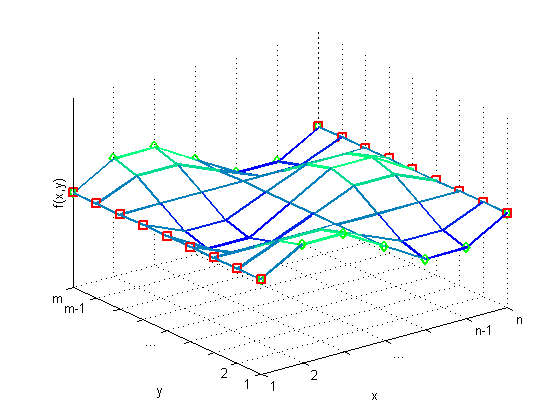
\includegraphics[width=0.8\textwidth]{LookupTable2D_periodic}
\end{figure}
For non-periodic signals there is no restriction regarding the last data points, see the example in the figure below.
\begin{figure}[H]
	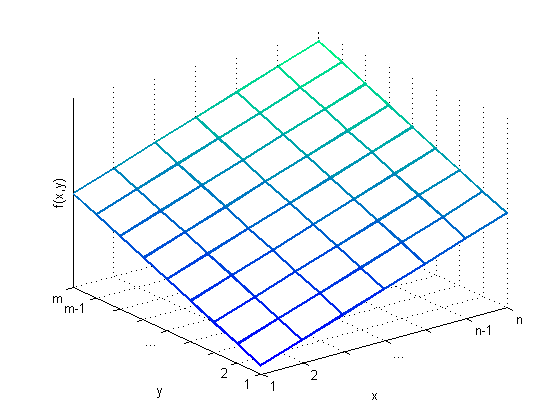
\includegraphics[width=0.8\textwidth]{LookupTable2D_non-periodic}
\end{figure}